% Put the project details here

\section{PROJECT DETAILS}
    International School Manila manages sponsorship billing and Letter of Guarantee coverage across PowerSchool (SIS), the Student Charging Portal, NetSuite (ERP), and the Online Billing System. The proposed system introduces a Sponsor Management layer that centralizes sponsor profiles, contacts, addresses, and LoG rules, then evaluates coverage at the point of charge entry. By deciding Covered / Not Covered once and propagating that decision to the ERP and statement layer, the design improves accuracy, reduces rework, and supports auditability.4
    
    %Steamline Overview
    \begin{figure}[ht]
    \begin{center}
        \vspace{4ex}
        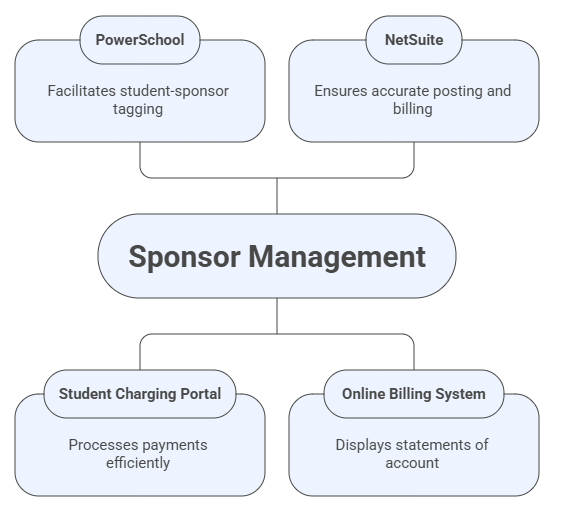
\includegraphics[width=300px]{Texfiles/images/streamline.png}
        \label{fig:Streamlining Sponsor Management}	
        \caption{Streamlining Sponsor Management}
    \end{center}
    \end{figure}
    
    PowerSchool provides sponsor tagging for students; NetSuite remains the posting and billing ledger; the Sponsor Management layer centralizes sponsor data and LoG rules; the Student Charging Portal handles charge entry and coverage evaluation; the Online Billing System publishes statements that reflect the final Bill-To and allocations.
    
        \subsection{Overview}   
        
        The implemented system delivers a web application that allows sponsors to self-service their details (name, TIN, addresses, multiple contacts), view a list of Letters of Guarantee per student per school year, and create or edit LoG entries through a guided modal form with status tracking. 

        %Context Diagram
        \begin{figure}[ht]
        \begin{center}
            \vspace{4ex}
            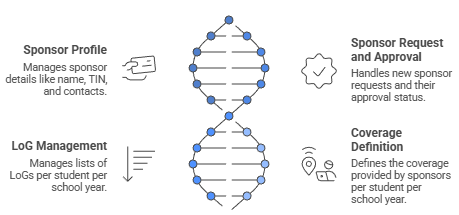
\includegraphics[width=400px]{Texfiles/images/Application Features.png}
            \label{fig:Application Features}	
            \caption{Application Features}
        \end{center}
        \end{figure} 
        
        For operators, the system provides real-time coverage preview within the Student Charging Portal and produces an explainable decision with reason codes.
        
        \subsection{Project Framework}
        
        Development followed a DevOps approach to deliver the ISM Sponsor Management and LoG Coverage Integration System through small, tested releases. Requirements and integration mappings were confirmed first, then features were built with automated builds, security checks, and end-to-end testing across PowerSchool, NetSuite, the Student Charging Portal, and the Online Billing System. Deployment used controlled rollouts with monitoring, audit logs, and continuous improvements based on feedback.
      
        \begin{enumerate}
            \item \textbf{Plan.}The first step is to confirm the end-to-end workflow and define the system boundaries. Requirements will be captured for sponsor onboarding and approval, sponsor master data propagation, student sponsor tagging, LoG creation per student per school year, and LoG coverage synchronization for billing. A role and permission matrix will be finalized for Admissions, Admin, Cashier, and Sponsor. Integration contracts will be documented, including field mappings, identifiers, timing expectations, error handling, and the source of truth for each record.
            \item \textbf{Design.} The solution will be designed as a role-based web application with distinct modules for Sponsor Profile, Sponsor Request and Approval, LoG Management, and Coverage Management. The integration design will specify how sponsor master data is published to each platform, how student \texttt{Sponsor\_OrgName} tagging is synchronized, and how LoG coverage is represented for NetSuite enrollment profiles. Security requirements will be built into the design, including server-side authorization, audit logging, and safe handling of attachments.
            \item \textbf{Build and Continuous Integration.} Development will be done in small increments that map to the business workflow, starting with sponsor onboarding and approval, then integrations, then LoG workflows, then coverage-to-billing outputs. A CI pipeline will run unit tests, linting, dependency scanning, and secret scanning on every change. Builds will be versioned and traceable, so any defect can be tied back to a specific change set.
            \item \textbf{Test.} Testing will be executed in a staging environment that mirrors production configuration as closely as possible. Functional testing will validate each role’s workflow, including approvals, sponsor list availability, student tagging sync, LoG creation and editing, and coverage completion. Integration testing will validate data movement and correctness across all systems using controlled test records. Security testing will focus on role isolation, data access controls, attachment validation, and audit log completeness. Non-functional testing will verify performance for search, listing, and modal workflows.
            \item \textbf{Release.} A release will be prepared only when test evidence shows the full sponsor-to-coverage workflow is stable. Release hardening will include configuration checks, environment variables and secrets validation, and confirmation of monitoring and logging. Release notes and rollback procedures will be documented, and go-live approvals will be obtained from the system owners.
            \item \textbf{Deploy.} Deployment will proceed from staging to production using a controlled rollout. Post-deploy smoke tests will confirm sponsor onboarding availability, sponsor list propagation signals, student tagging synchronization, and LoG coverage creation. Rollback will be immediately available if integrations or core workflows fail.
            \item \textbf{Operate and Monitor.} After deployment, monitoring will focus on application health, synchronization success rates, and data consistency signals that indicate mismatches across platforms. Audit logs will be reviewed for approvals and record changes, and alerts will be tuned for integration failures that could affect billing readiness. Operational runbooks will document how to respond to sync failures, data mismatches, and user access issues.
            \item \textbf{Feedback and Improve.} User feedback from Admissions, Admin, Cashier, and Sponsors will be collected to identify friction points and missing validations. Support issues and monitoring trends will drive improvements to workflow clarity, integration reliability, and test coverage. Enhancements will be delivered through the same controlled pipeline, ensuring continuous improvement without breaking billing-critical processes.
        \end{enumerate}

        \subsection{Materials/Technologies Used}
        The proposed solution uses a Microsoft Azure–based technology stack to support secure, scalable development and reliable integration across PowerSchool, NetSuite, the Student Charging Portal, and the Online Billing System.
        \begin{itemize}
            \item \textbf{Application Backend.} Built on \textbf{.NET (ASP.NET Core)} with secured \textbf{REST APIs} published via \textbf{Azure API Management}. Background sync and validation jobs run on \textbf{Azure Functions}, with secrets stored in \textbf{Azure Key Vault} and delivery automated through \textbf{Azure DevOps} pipelines.
            \item \textbf{Database Layer.} Uses \textbf{Azure SQL (MSSQL)} to store sponsor records, contacts, LoG and coverage data, sync status, and audit logs.
            \item \textbf{Web Front-end.} Implemented as an \textbf{ASP.NET Core MVC + PWA} interface with role-based pages for Sponsors and staff, using \textbf{Azure AD} authentication with optional \textbf{Google OAuth}.
            \item \textbf{Monitoring and Operations}. Uses \textbf{Azure Monitor} and \textbf{Application Insights} for performance, logs, alerts, and integration health monitoring through \textbf{API Management} and Function telemetry.
            \item \textbf{Verification Aids.} Uses \textbf{Azure DevOps} test pipelines, staging smoke tests, and repeatable validation scripts to confirm sponsor sync, student tagging sync, and LoG coverage outputs.
        \end{itemize}

 
        \subsection{System Design}
        Functionally, the system covers: sponsor master data management; LoG rule authoring per sponsor and per student; coverage evaluation for charge lines; audit logging of every decision; and synchronized identifiers for PowerSchool, SCP, NetSuite, and OBS. Non-functional requirements emphasize security (SSO, RBAC, audit), performance (sub-second coverage preview for common items), and maintainability.

        \begin{itemize}
            \item \subsubsection{Architecture overview.} The system is designed as a role-based web application on Microsoft Azure that centralizes sponsor master data and LoG coverage rules, then synchronizes validated identifiers and outcomes to PowerSchool, NetSuite, the Student Charging Portal, and the Online Billing System. The solution uses an ASP.NET Core backend for business logic and integrations, an ASP.NET Core MVC front end with PWA capabilities for role-based access, and Azure SQL (MSSQL) as the primary data store. External integration traffic is governed through Azure API Management, while scheduled synchronization and coverage evaluation tasks run as Azure Functions.
            %Architecture overview
            \begin{figure}[ht]
            \begin{center}
                \vspace{4ex}
                \includegraphics[width=400px]{Texfiles/images/Architecture overview.png}
                \label{fig:Architecture overview}	
                \caption{Architecture overview}
            \end{center}
            \end{figure}     
            \item \subsubsection{Core functional services.} The application provides five core services. Sponsor Master Data Management maintains sponsor identity, TIN, addresses, and contacts with controlled updates and approval support where required. LoG Rule Authoring supports rule definition per sponsor and per student, enabling differentiated coverage policies. Coverage Evaluation applies LoG rules to charge line items to determine covered and bill-to outcomes, including a fast preview path for common items. Decision Auditing records every evaluation decision with inputs, rule version, reason, user context, and timestamp. Identifier Synchronization ensures consistent sponsor and student identifiers across PowerSchool, SCP, NetSuite, and OBS to prevent mismatched coverage behavior.
            \item \subsubsection{Data model and persistence.} Azure SQL stores sponsor master records, contact records, LoG rule definitions, rule versions, effective date ranges, student-specific overrides, LoG instances per student per school year, and coverage results used by downstream billing. Audit log tables capture every decision and key user action, including before-and-after values for changes. Integration tracking tables store sync status, last successful timestamps, retries, and error details to support operational visibility.
            \item \subsubsection{Coverage Computation and Bill-To Determination.} The system evaluates sponsorship coverage at the charge line level using deterministic rules derived from the sponsor’s LoG and any student-specific overrides. Each evaluation produces a coverage classification, an authoritative Bill-To designation, sponsor–parent allocation amounts and percentages, and an auditable explanation containing the applicable rule version and reason code.
            Inputs to the evaluation include Student Identifier, Sponsor Identifier, School Year, Charge Item Code, Charge Category, Charge Amount, Charge Date, LoG effective date range, coverage caps or limits, exclusions, required documentation flags, and student-level overrides. The evaluation enforces rule priority to prevent ambiguous or conflicting outcomes.
            
            Coverage outcomes are classified as: (a) Covered, where the sponsor is responsible for the full amount subject to caps and effective dates; (b) Split, where sponsor and parent share responsibility based on rule-defined allocation; and (c) Not Covered, where the parent is responsible for the full amount.
            
            Allocation computation is performed using explicit formulas. For cap-based splits, the system computes SponsorCoveredAmount = min(ChargeAmount, RemainingCap) and ParentAmount = ChargeAmount - SponsorCoveredAmount. Percent allocations are computed as SponsorPercent = SponsorCoveredAmount / ChargeAmount and ParentPercent = ParentAmount / ChargeAmount. The system records both the monetary and percentage allocations to support downstream billing and reconciliation.
            
            Bill-To designation is derived from the computed allocation. If SponsorPercent equals 
            1.00, Bill-To is Sponsor. If SponsorPercent equals 0.00, Bill-To is Parent. If SponsorPercent is between 0.00 and 1.00, Bill-To is Split and the system propagates explicit sponsor and parent allocations to downstream systems. Each decision is persisted with a reason code and rule version to ensure traceability and auditability.
 
            \item \subsubsection{Integration design.} This sequence diagram shows the real-time interaction across systems when a charge is entered. The Student Charging Portal calls the Coverage API for a preview decision. The Coverage API reads LoG and rule data from the Sponsor Master, returns a decision with allocations and audit metadata, then the portal posts allocations to NetSuite and updates the Online Billing System for statement display.
            
            %Integration Interaction Flow
            \begin{figure}
                \centering
                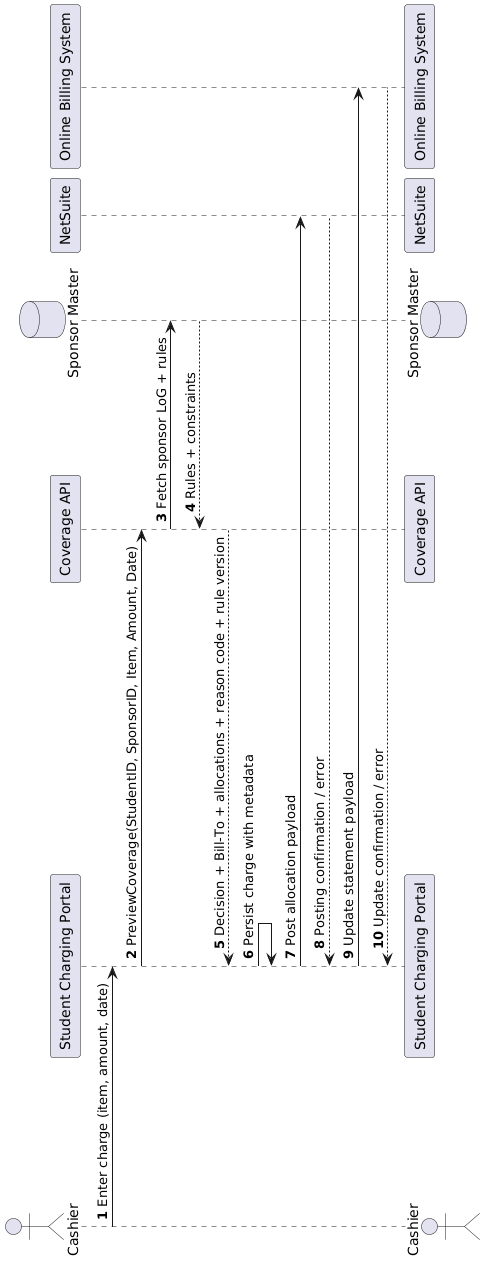
\includegraphics[width=0.5\linewidth]{Texfiles/images/integration flow.png}
                \caption{Integration Interaction Flow}
                \label{fig:Integration Interaction Flow}
            \end{figure}

            %Sponsor Management ERD
            \begin{figure}
                \centering
                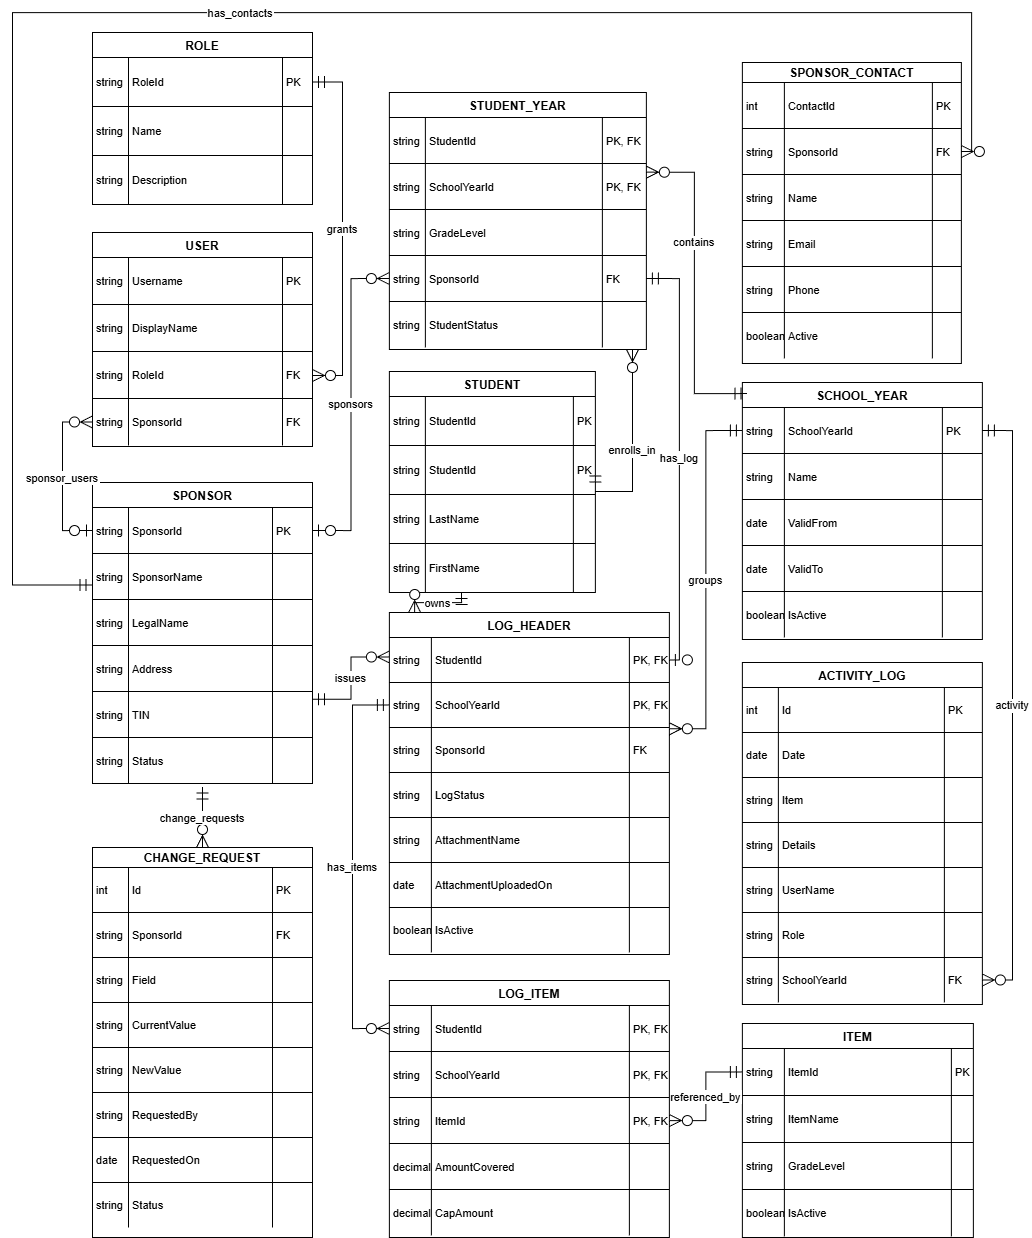
\includegraphics[width=1\linewidth]{Texfiles/images/Proposal ERD.png}
                \caption{Sponsor Management ERD}
                \label{fig:Sponsor Management ERD}
            \end{figure}
            \pagebreak

            \item \subsubsection{Per-Application Activity Diagram.} 
            \textbf{Powerschool Activity (Student Record and Sponsor Tagging).} This activity diagram describes how PowerSchool serves as a source of student identity and sponsor linkage. Staff create or update student records, assign a SponsorID or sponsorship indicator, validate sponsor association, and sync the student-sponsor relationship to the Sponsor Master. When no sponsor is linked, the student remains parent-responsible by default. 
            
            %PS Activity
            \begin{figure}[ht]
            \begin{center}
                \vspace{4ex}
                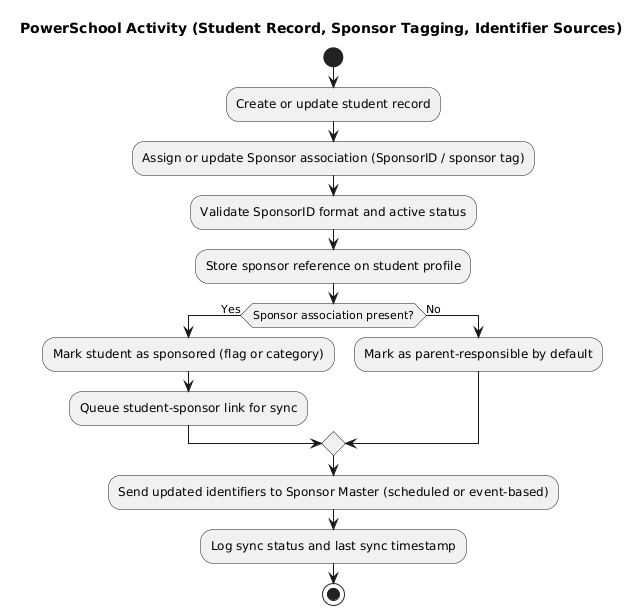
\includegraphics[width=350px]{Texfiles/images/PS Activity.png}
                \label{fig:PowerSchool Activity}	
                \caption{PowerSchool Activity}
            \end{center}
            \end{figure}
            \pagebreak

            \textbf{Student Charging Portal Activity (Charge Entry and Coverage Preview).} This activity diagram shows how the Student Charging Portal supports decision-making at the point of charge entry. The user inputs charge details, requests a coverage preview, and receives a coverage decision with sponsor and parent allocations. If the user accepts the decision, the charge is committed with decision metadata and posted to downstream systems. If not, the user adjusts inputs and reruns the preview. 

            %Student Charging Portal Activity
            \begin{figure}[ht]
            \begin{center}
                \vspace{4ex}
                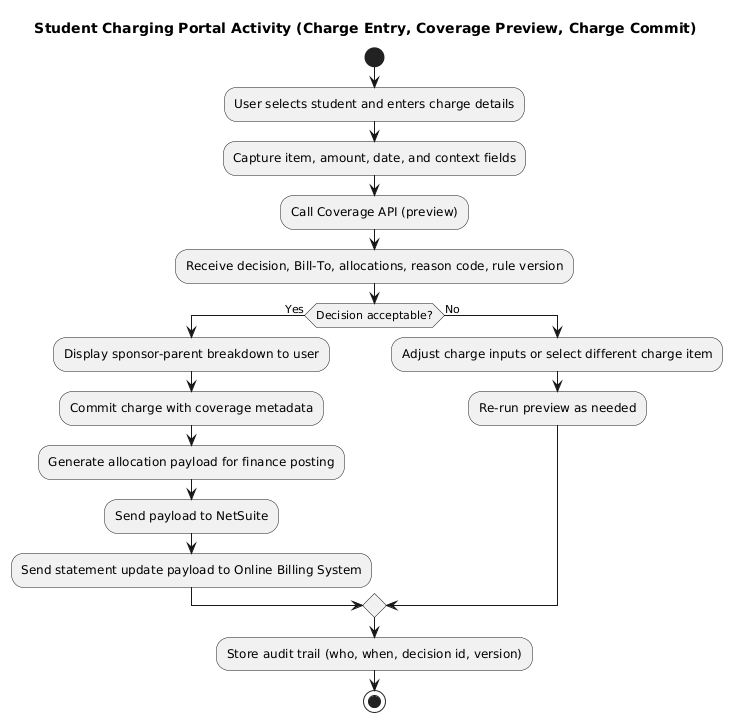
\includegraphics[width=350px]{Texfiles/images/SCP Activity.png}
                \label{fig:Student Charging Portal Activity}	
                \caption{Student Charging Portal Activity}
            \end{center}
            \end{figure}
            \pagebreak

            \textbf{NetSuite Activity (Allocation Posting and Receivables).} This activity diagram explains how NetSuite receives allocation results and records them as receivables. NetSuite validates the payload, creates AR transaction lines for sponsor and parent portions, attaches the decision metadata for auditability, and returns confirmation. Invalid payloads are rejected with error details and logged for troubleshooting. 
            
            %Netsuite Activity
            \begin{figure}[ht]
            \begin{center}
                \vspace{4ex}
                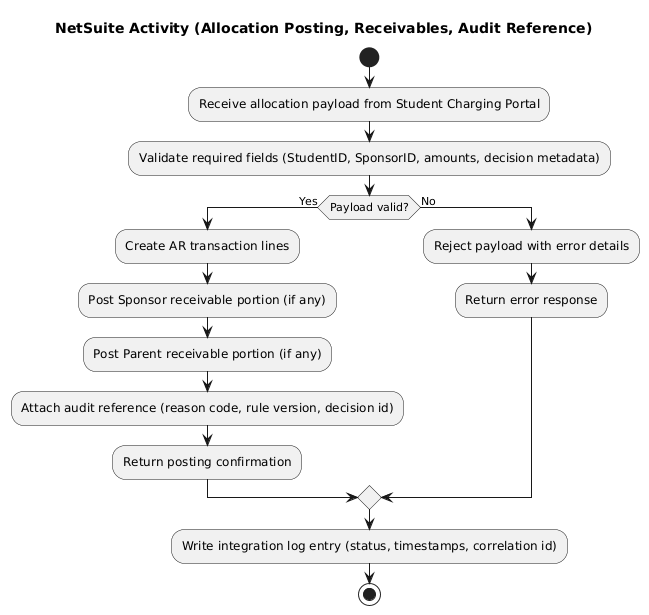
\includegraphics[width=350px]{Texfiles/images/Netsuite Activity.png}
                \label{fig:Netsuite Activity}	
                \caption{Netsuite Activity}
            \end{center}
            \end{figure}
            \pagebreak

            \textbf{Online Billing System Activity (Statement Presentation).} This activity diagram shows how the Online Billing System presents the billing outcome to end users. It receives statement updates, validates the update, applies charge lines and sponsor-parent allocations, and publishes the updated statement. It also records revision history and integration correlation identifiers for traceability. 
            
            %Online Billing System Activity
            \begin{figure}[ht]
            \begin{center}
                \vspace{4ex}
                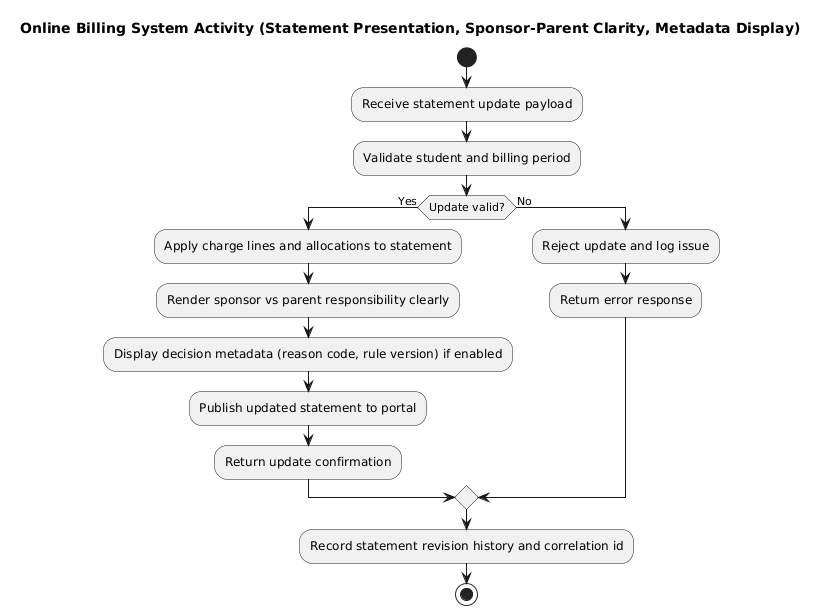
\includegraphics[width=350px]{Texfiles/images/Online Billing System Activity.png}
                \label{fig:Online Billing System Activity}	
                \caption{Online Billing System Activity}
            \end{center}
            \end{figure}
            \pagebreak

            \item \subsubsection{Cross-System Data Mapping and ERD Integration View.} The integration view should identify the canonical identifiers used to link student, sponsor, charge, and allocation records across systems. Where vendor schemas are proprietary or inaccessible, the manuscript may present a logical ERD integration view that emphasizes join keys, mapping fields, and synchronization directionality.

            \begin{center}
            \captionsetup{type=table}
            \caption{Logical cross-system entity mapping and key identifiers}
            \label{table:role-functions}
            \smalltable
            \scriptsize
            \begin{tabular}{|>{\raggedright\arraybackslash}p{2.6cm}|
                            >{\raggedright\arraybackslash}p{1.8cm}|
                            >{\raggedright\arraybackslash}p{2.6cm}|
                            >{\raggedright\arraybackslash}p{2.6cm}|
                            >{\raggedright\arraybackslash}p{2.6cm}|}
            \hline
            \textbf{Entity}&
            \textbf{PowerSchool (SIS)}&
            \textbf{Student Charging Portal}&
            \textbf{NetSuite (ERP)}&
            \textbf{Online Billing System}
            \\
            \hline\hline
            
            \textbf{Student}&
            StudentID (authoritative)&
            StudentID (reference)&
            Customer/Student key (mapped)&
            Student account key (mapped)
            \\
            \hline
            
            \textbf{Sponsor}&
            Sponsor reference (if present)&
            SponsorID (reference)&
            CustomerID (mapped)&
            Sponsor account key (mapped)
            \\
            \hline
            
            \textbf{LoG}&
            Document reference (optional)&
            LoG record (reference)&
            Not stored as LoG (reference via audit id)&
            Displayed metadata (reference)
            \\
            \hline
            
            \textbf{Charge Line}&
            Optional fee definition&
            ChargeLineID (authoritative at entry)&
            Transaction/Invoice line key (mapped)&
            Statement line key (mapped)
            \\
            \hline
            
            \textbf{Allocation}&
            Not computed&
            Allocation fields (authoritative)&
            Accounting split fields (mapped)&
            Displayed split fields (mapped)
            \\
            \hline
          
            \end{tabular}
            \end{center}
            % --- END ---
            
            \item \subsubsection{Workflow alignment.} Sponsor onboarding begins with staff creation or submission of sponsor details and required documentation, followed by approval where applicable. Upon approval, sponsor identifiers are integrated and made available in PowerSchool and downstream systems. Student sponsor assignment is driven by \texttt{Sponsor\_OrgName} tagging in PowerSchool and synchronized to NetSuite, OBS, and SCP. LoG rules and student-level LoG coverage are authored and maintained within the application, then evaluated against charge line items to produce coverage decisions that are recorded and synchronized for billing use.
            
            %Context Diagram
            \begin{figure}[ht]
            \begin{center}
                \vspace{4ex}
                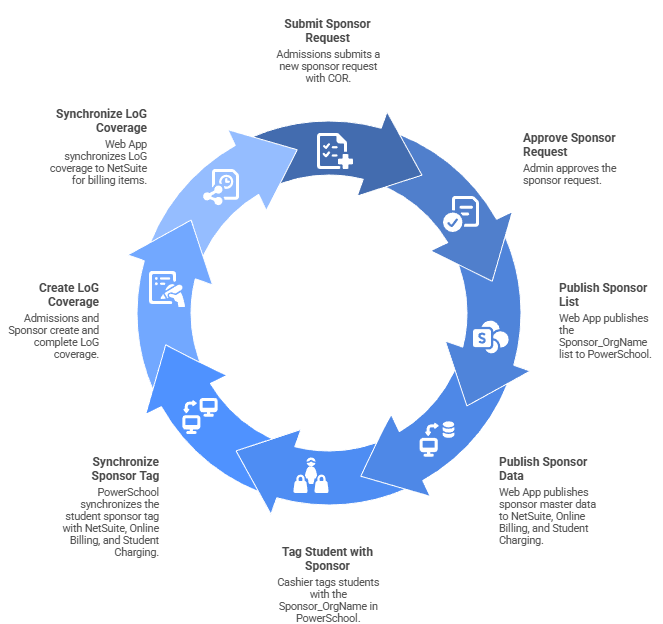
\includegraphics[width=400px]{Texfiles/images/Context Diagram.png}
                \label{fig:Context Diagram}	
                \caption{Context Diagram}
            \end{center}
            \end{figure} 
        \end{itemize}
        \pagebreak
        
        \subsection{Implementation}
        The initial implementation focuses on three threads in parallel:

        \begin{enumerate}
            \item Sponsor Master CRUD with contacts and addresses, including uniqueness checks for name/TIN and cross-system IDs.
            \item LoG Modal for create/edit with per-student rules, caps, and effective dates, plus status changes and notes.
            \item Coverage API that evaluates a mock charge line and returns a decision with reason codes and audit entries.
        \end{enumerate}

        Deployment uses Azure DevOps pipelines (Build → Test → Deploy to Dev → Manual Approval → Deploy to Pilot). Pilot data uses de-identified records. Success is measured by reduced manual checks, fewer reversals, and consistent Bill-To assignment at invoice creation.

        \subsection{User Interface Wireframe}
        The Sponsor Management prototype presents a role-based workflow for maintaining sponsor records, managing Letters of Guarantee (LoGs), and coordinating sponsor-driven updates. Each role interacts with the same core pages, but the system emphasizes different tasks based on operational responsibility. The following sections describe each role’s typical functions and the screens that support them.
        \pagebreak

        \begin{center}
        \captionsetup{type=table}
        \caption{Role Functions}
        \label{table:role-functions}
        \smalltable
        \scriptsize
        \begin{tabular}{|>{\raggedright\arraybackslash}p{2.6cm}|
                        >{\raggedright\arraybackslash}p{2.0cm}|
                        >{\raggedright\arraybackslash}p{2.6cm}|
                        >{\raggedright\arraybackslash}p{2.6cm}|
                        >{\raggedright\arraybackslash}p{2.6cm}|}
        \hline
        \textbf{Module} &
        \textbf{Admin} &
        \textbf{Admissions} &
        \textbf{Cashier} &
        \textbf{Sponsor} \\
        \hline\hline
        
        \textbf{Login} &
        Sign in &
        Sign in &
        Sign in &
        Sign in \\
        \hline
        
        \textbf{Dashboard} &
        Monitor totals, oversee requests &
        Check totals, review pending updates &
        Quick LoG volume check &
        Optional, limited \\
        \hline
        
        \textbf{Sponsor Profile} &
        Add and edit sponsors, review requests &
        Search, add, edit sponsors &
        Lookup sponsor details &
        View profile, view contacts, request changes \\
        \hline
        
        \textbf{Letters of Guarantee} &
        Full access, deactivate or reactivate &
        Confirm coverage alignment &
        Verify status and attachments, view coverage &
        Review coverage status \\
        \hline
        
        \textbf{Reports} &
        Oversight reports &
        Tracking reports &
        Reconciliation support &
        View if enabled \\
        \hline
        
        \textbf{Settings} &
        Manage school years, students, items, roles, users &
        Not typical &
        Not typical &
        Not available \\
        \hline
        
        \end{tabular}
        \end{center}
        % --- END ---
        
        This guide explains how to navigate the Sponsor Management interface and complete routine tasks. It focuses on sponsor search, sponsor record maintenance, contact viewing, and sponsor change requests. It also explains core navigation features such as the school year selector and switching between modules.
        
        \begin{figure}
        \centering
        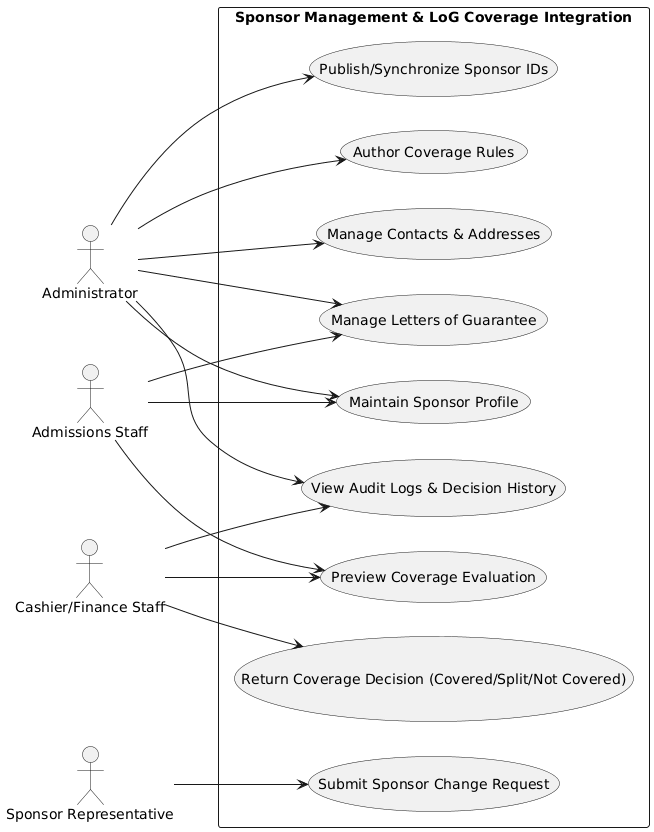
\includegraphics[width=0.75\linewidth]{Texfiles/images/Role Function Diagram.png}
        \caption{Role Function Diagram}
        \label{fig:Role Function Diagram}
        \end{figure}
        \pagebreak
        
        The interface is role-based. The supported roles are Admin, Admissions, Cashier, and Sponsor. Each role has different viewing and action permissions across modules.

        \begin{enumerate}
            \item \textbf{Signing in}
                \begin{itemize}
                    \item Open the login pagel
                    \item Enter a username and password.
                    \item Select \textbf{Sign in} to proceed.
                    \item Use any of the provided training accounts shown on the login screen.
                \end{itemize}
                %Login
                \begin{figure}[ht]
                \begin{center}
                    \vspace{4ex}
                    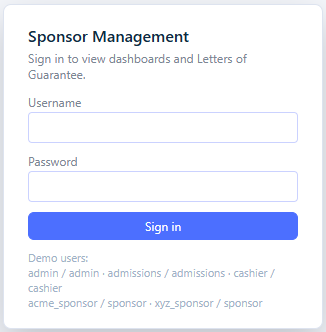
\includegraphics[width=200px]{Texfiles/images/Login.png}
                    \label{fig:Login}	
                    \caption{Login}
                \end{center}
                \end{figure}
                \pagebreak
            \item \textbf{Orientation to the interface}
                \begin{itemize}
                    \item \textbf{Top bar Controls}
                    The top bar displays the signed-in user’s role and name, provides a \textbf{Logout} button, and includes a \textbf{School year} selector for switching the active school year view.
                    \item \textbf{Page navigation}
                    After login, the user lands on the \textbf{Dashboard}. From the sidebar navigation, the user can open other modules such as:
                        \begin{itemize}
                            \item \textbf{Sponsor Profile}
                            \item \textbf{Letters of Guarantee}
                            \item \textbf{Reports}
                            \item \textbf{Settings} (role-dependent access)
                        \end{itemize}
                    %Interface
                    \begin{figure}[ht]
                    \begin{center}
                        \vspace{4ex}
                        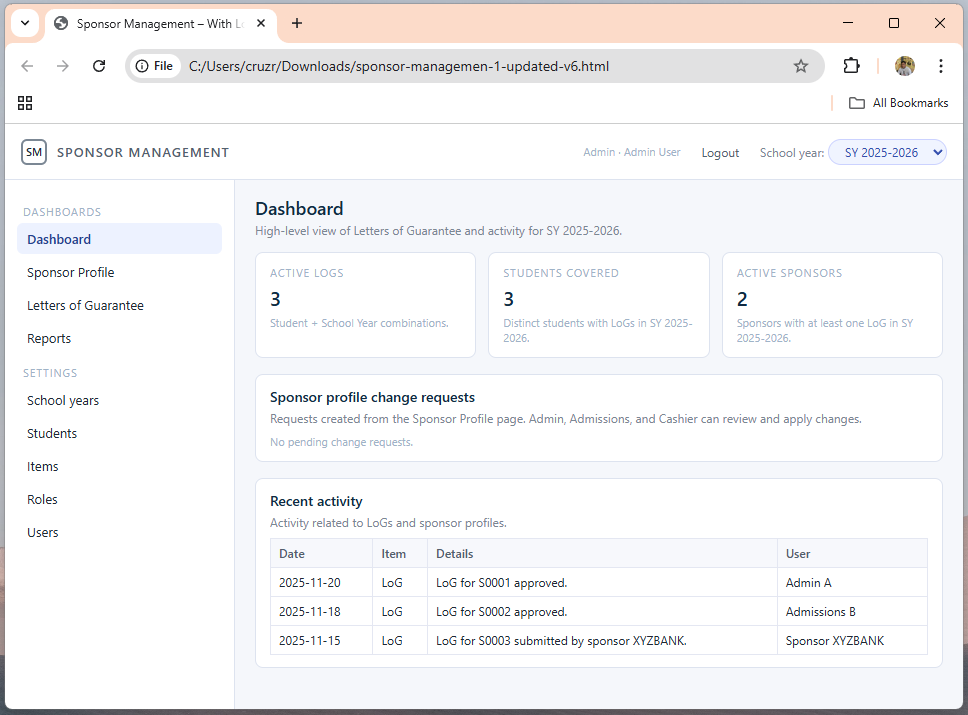
\includegraphics[width=400px]{Texfiles/images/Interface.png}
                        \label{fig:Interface}	
                        \caption{Interface}
                    \end{center}
                    \end{figure}
                \end{itemize}
            \item \textbf{Dashboard module (Landing page for all roles)}
            The Dashboard is the first page shown after login for Admin, Admissions, Cashier, and Sponsor users. It provides high-level metrics for the selected school year, including counts such as Active LoGs and Students covered. Staff views also surface pending change request counts for follow-up.
            \item \textbf{Sponsor Profile module}
            The Sponsor Profile module contains official sponsor information, sponsor contacts, and sponsor change request functionality.
            %sponsor profile
            \begin{figure}[ht]
            \begin{center}
                \vspace{4ex}
                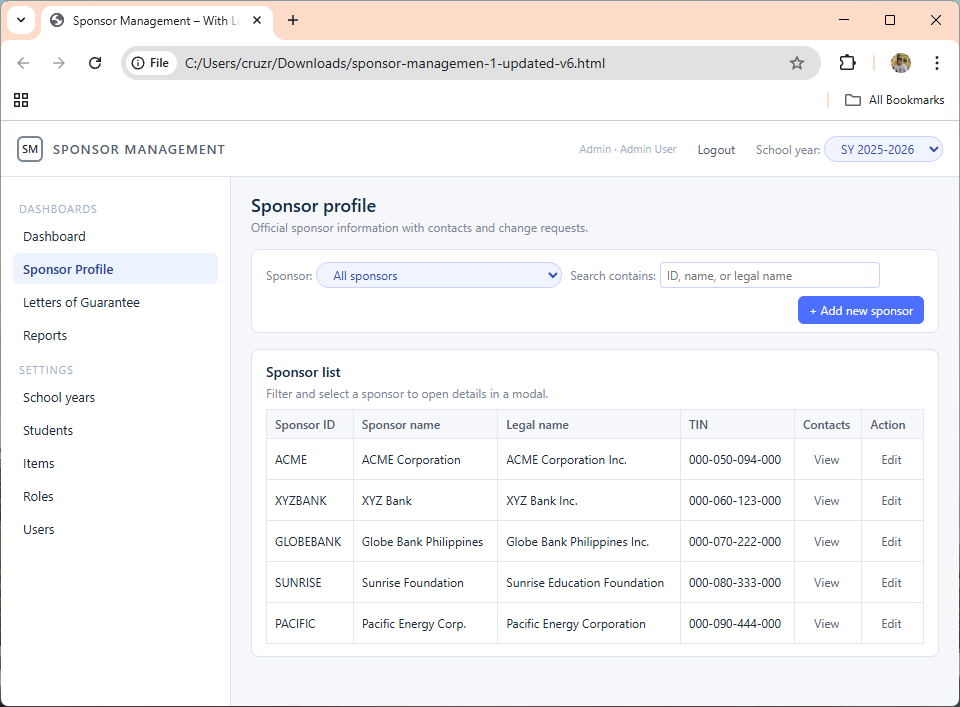
\includegraphics[width=400px]{Texfiles/images/sponsor profile.png}
                \label{fig:sponsor profile}	
                \caption{sponsor profile}
            \end{center}
            \end{figure}
            %sponsor new
            \begin{figure}[ht]
            \begin{center}
                \vspace{4ex}
                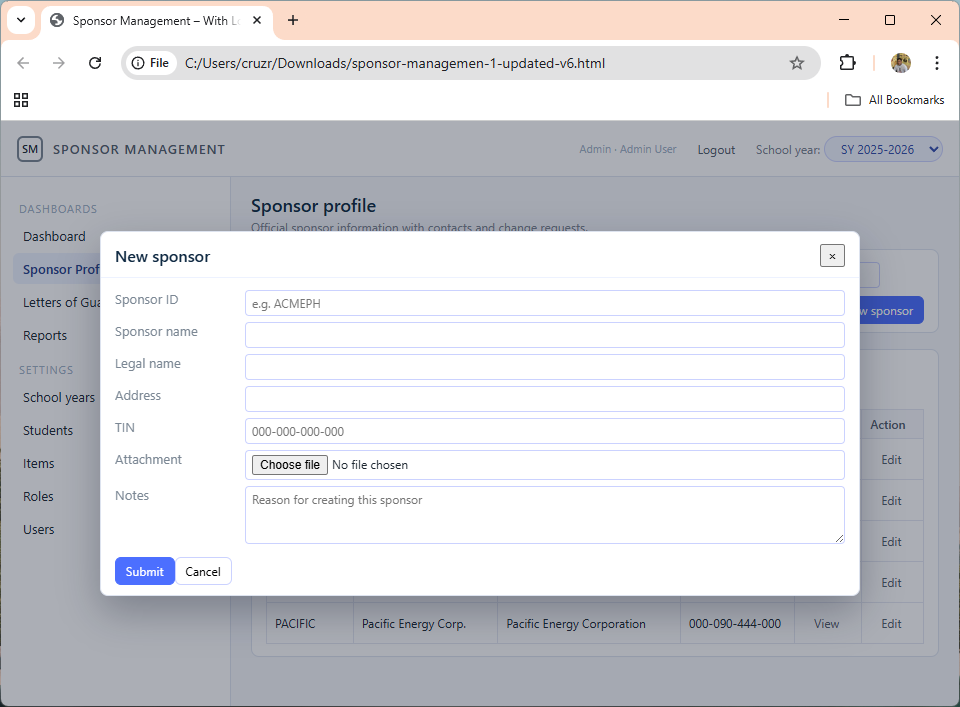
\includegraphics[width=400px]{Texfiles/images/sponsor new.png}
                \label{fig:Sponsor new}	
                \caption{Sponsor new}
            \end{center}
            \end{figure}
            \begin{itemize}
                \item \textbf{Staff workflow: Search, filter, and add a sponsor}
                Staff users see a filter bar with:
                    \begin{itemize}
                        \item \textbf{Sponsor} dropdown (All sponsors or a selected sponsor)
                        \item \textbf{Search contains} field (ID, name, or legal name)
                        \item + \textbf{Add new sponsor} button
                    \end{itemize}
                The + Add new sponsor button is right-aligned with the Sponsor and Search fields.
                \item \textbf{Staff workflow: View and edit sponsor records}
                Staff users can review a sponsor list table (Sponsor ID, Sponsor name, Legal name, TIN, Contacts, Action). Staff can open contacts and use the \textbf{Edit} action to update sponsor fields, then select \textbf{Save} or \textbf{Cancel}.
                \item \textbf{Staff workflow: Add a new sponsor}
                    \begin{itemize}
                        \item Select + \textbf{Add new sponsor}.
                        \item Complete the form fields (Sponsor ID, Sponsor name, Legal name, Address, TIN).
                        \item Optionally add an attachment and notes.
                        \item Select \textbf{Submit} to create the sponsor, or \textbf{Cancel} to exit.
                    \end{itemize}
                \item \textbf{Sponsor workflow: View sponsor information and contacts}
                Sponsor users see a Sponsor Information table that includes Sponsor ID, Sponsor name, Legal name, Address, TIN, and action buttons for \textbf{View contacts} and \textbf{Request change}.
                \item \textbf{Sponsor workflow: Submit a change request}
                    \begin{itemize}
                        \item Select \textbf{Request change}.
                        \item Choose the field to update (Sponsor name, Legal name, Address, or TIN).
                        \item Review the current value and enter the requested value.
                        \item Select \textbf{Submit request} to send the request, or \textbf{Cancel} to close the form.
                    \end{itemize}
                \end{itemize}
            \item \textbf{Letters of Guarantee module}
            The Letters of Guarantee module lists LoGs by student and school year. It includes search and filtering logic and supports opening detailed coverage views.
            %Letter of Guarantee
            \begin{figure}[ht]
            \begin{center}
                \vspace{4ex}
                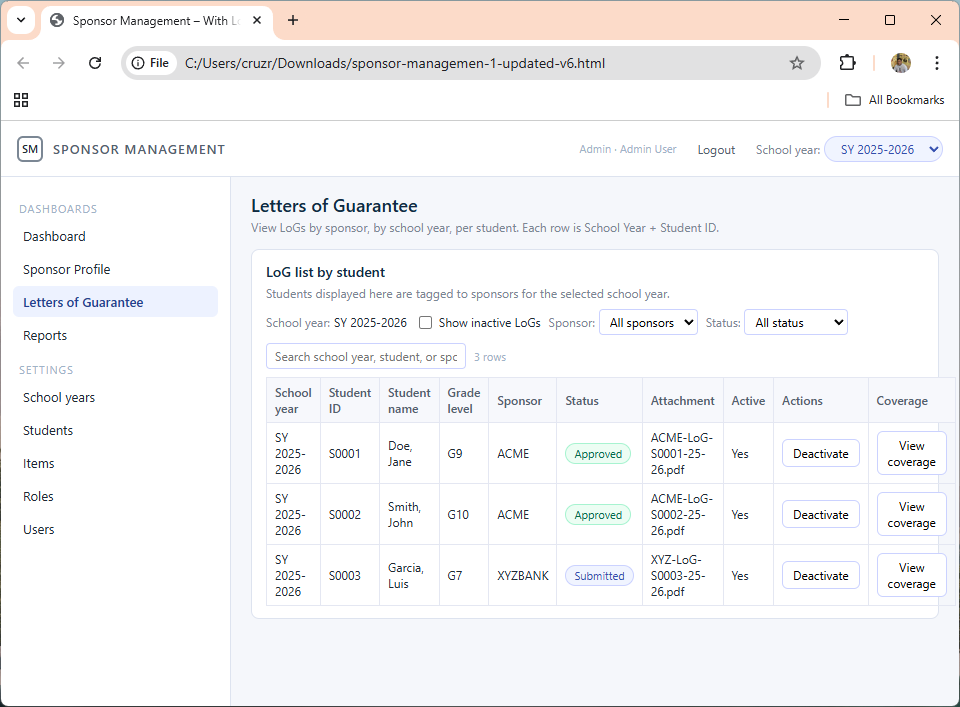
\includegraphics[width=400px]{Texfiles/images/LoG.png}
                \label{fig:Letter of Guarantee}	
                \caption{Letter of Guarantee}
            \end{center}
            \end{figure}
            \begin{itemize}
                \item \textbf{Search and view LoG rows} Users can search within the list and review columns such as School year, Student ID, Student name, Grade level, Sponsor, Status, Attachment, Active, and Coverage.
                %LoG Coverage
                \begin{figure}[ht]
                \begin{center}
                    \vspace{4ex}
                    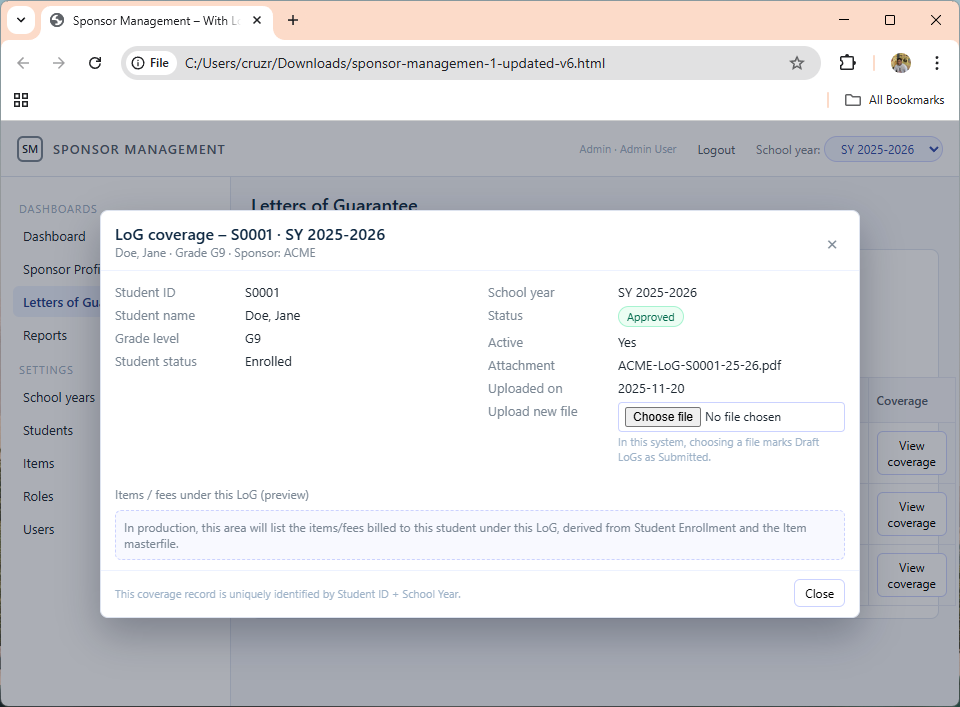
\includegraphics[width=400px]{Texfiles/images/LoG Coverage.png}
                    \label{fig:LoG Coverage}	
                    \caption{LoG Coverage}
                \end{center}
                \end{figure}
                \item \textbf{Administrative actions} Admin users can toggle activation status using \textbf{Deactivate} or \textbf{Reactivate}. Any user can select \textbf{View coverage} to open a coverage view for the selected row.
            \end{itemize}
            \pagebreak
            \item \textbf{Settings module}
            \begin{itemize}
                \item \textbf{School Years} It supports adding and editing school year records, defining valid date ranges, and setting the active school year context for viewing and reporting.
                \item \textbf{Students} The Students page supports viewing students by school year, sponsor, and status. It provides filters and a search field for student ID or name, plus an action to \textbf{+ Add student}.
                \item \textbf{Items} It supports adding and editing items, assigning grade-level applicability where required, and enabling or disabling items for use in LoG coverage evaluation.
                \item \textbf{Roles} The Roles page includes an \textbf{Add role} action and a role definitions table for reviewing and maintaining role records.
                \item \textbf{Users} It supports creating and editing users, assigning roles, linking sponsor users to a sponsor record where applicable, and managing credentials for training or controlled access scenarios.
            \end{itemize}
            %school year
            \begin{figure}[ht]
            \begin{center}
                \vspace{4ex}
                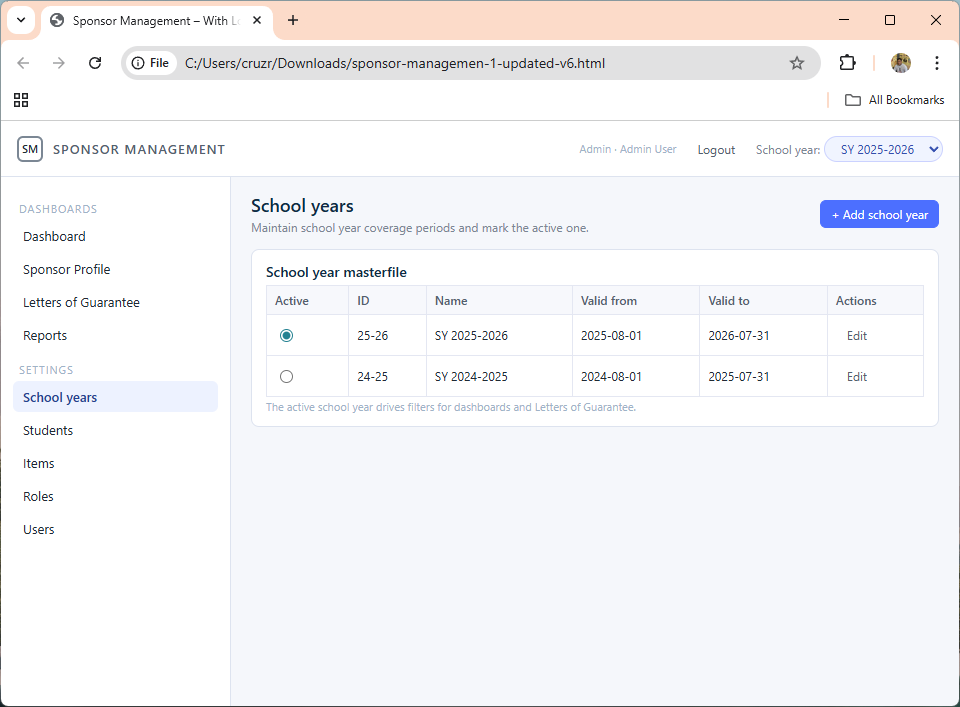
\includegraphics[width=400px]{Texfiles/images/school year.png}
                \label{fig:School Year}	
                \caption{School Year}
            \end{center}
            \end{figure}
            %Students
            \begin{figure}[ht]
            \begin{center}
                \vspace{4ex}
                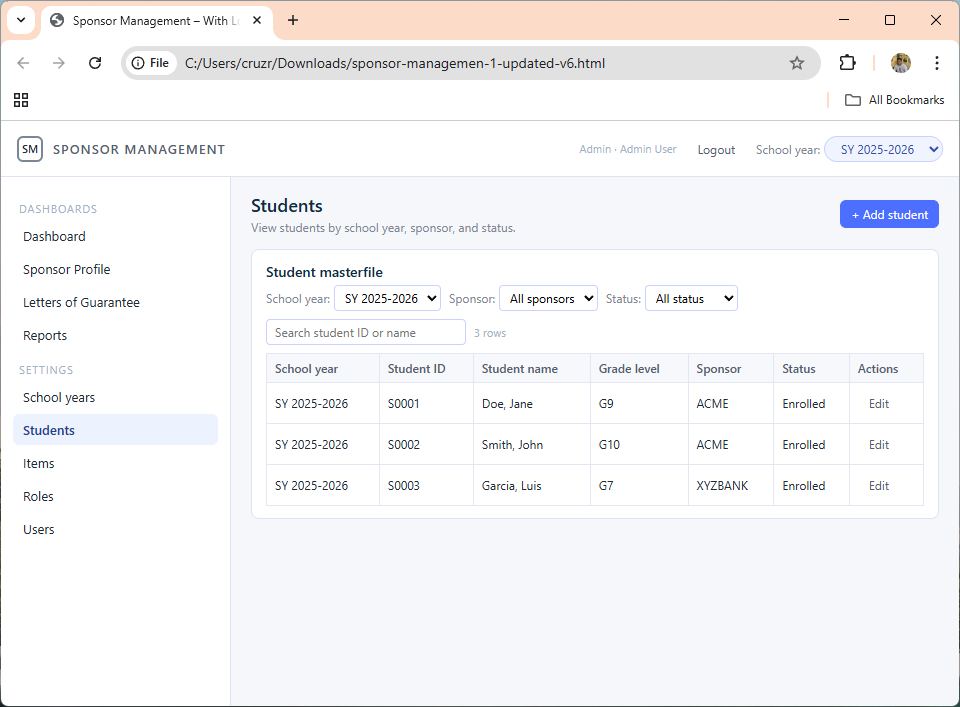
\includegraphics[width=400px]{Texfiles/images/students.png}
                \label{fig:Students}	
                \caption{Students}
            \end{center}
            \end{figure}
            %Items
            \begin{figure}[ht]
            \begin{center}
                \vspace{4ex}
                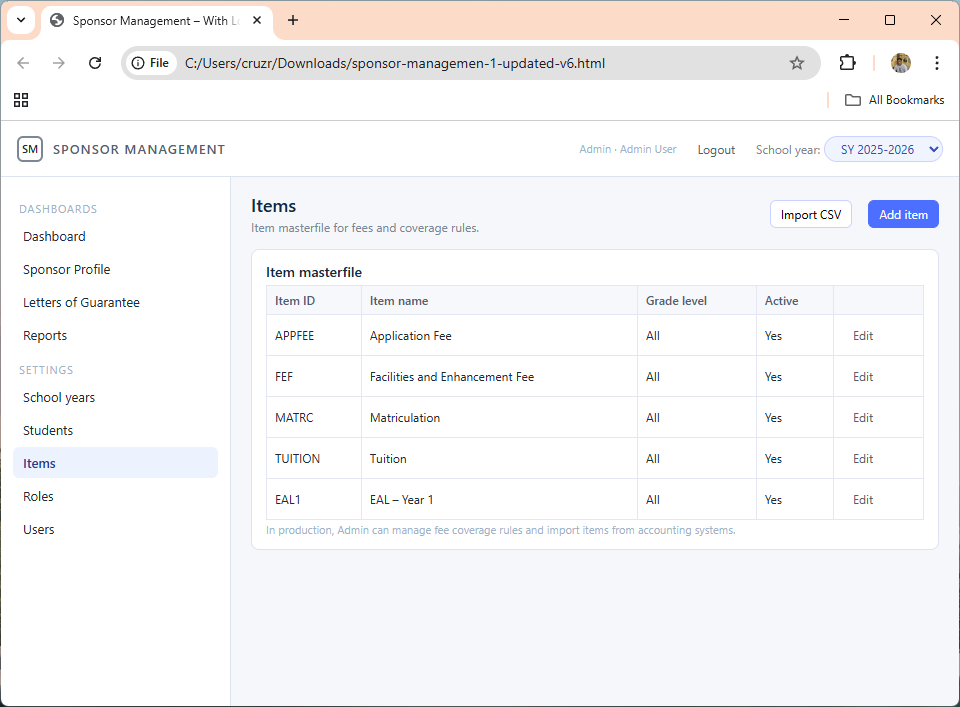
\includegraphics[width=400px]{Texfiles/images/items.png}
                \label{fig:Items}	
                \caption{Items}
            \end{center}
            \end{figure}
            %Roles
            \begin{figure}[ht]
            \begin{center}
                \vspace{4ex}
                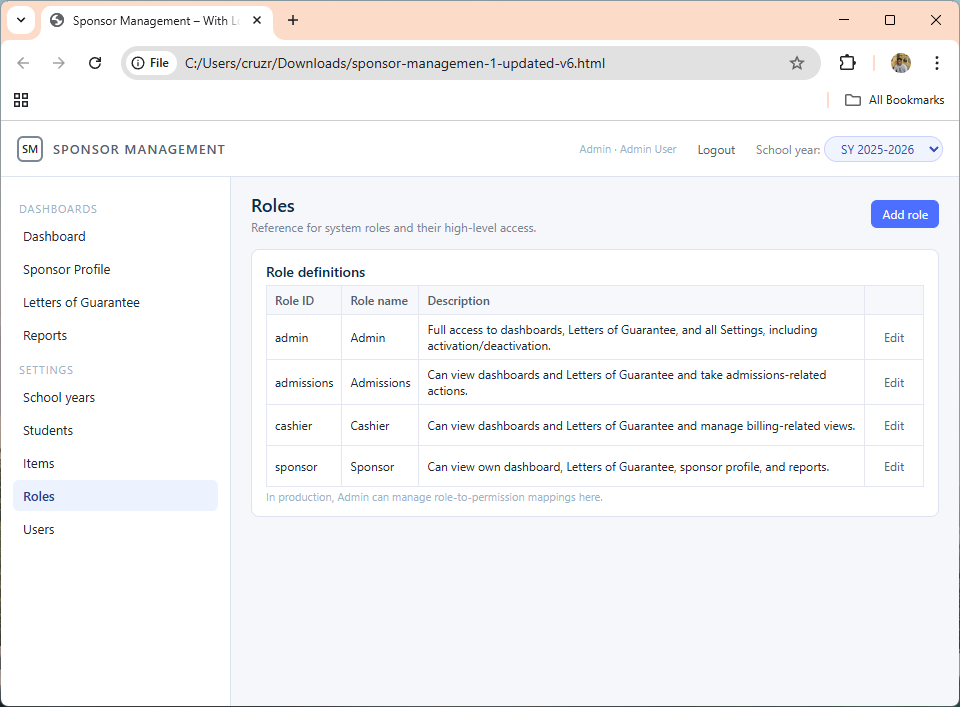
\includegraphics[width=400px]{Texfiles/images/roles.png}
                \label{fig:Roles}	
                \caption{Roles}
            \end{center}
            \end{figure}
            %Users
            \begin{figure}[ht]
            \begin{center}
                \vspace{4ex}
                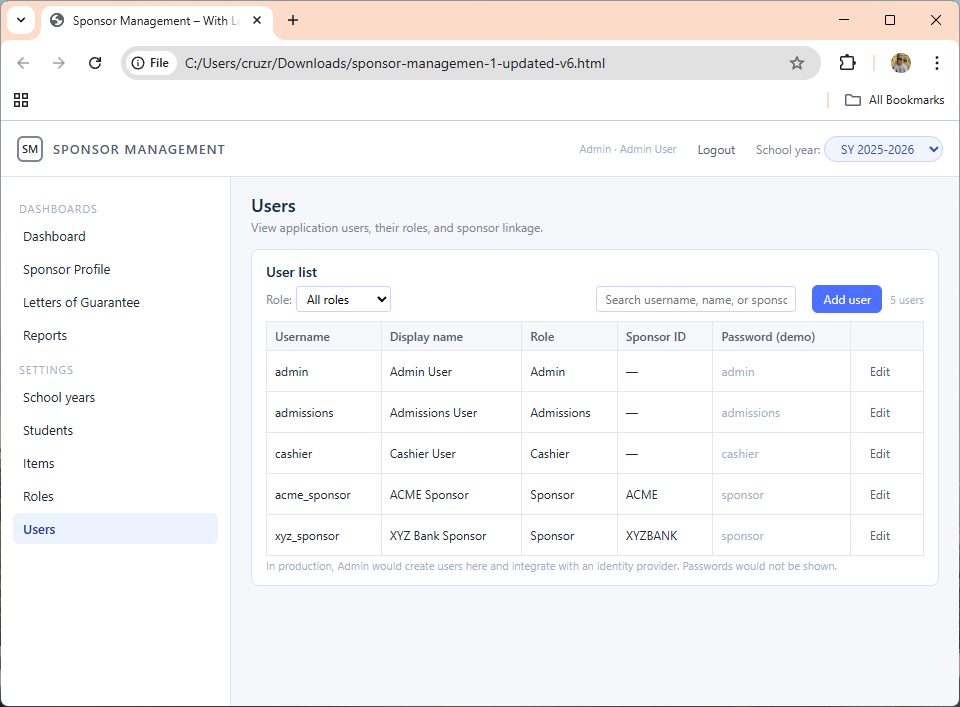
\includegraphics[width=400px]{Texfiles/images/users.png}
                \label{fig:Users}	
                \caption{Users}
            \end{center}
            \end{figure}    
        \end{enumerate}

        